% 2023本郷祭 マイコン部 部誌 「マイコンHONGOMagazine」 TeXテンプレート

% =環境設定=

\documentclass[b5paper,9pt,platex,dvipdfmx]{jsarticle}

% 数式
\usepackage{amsmath,amsfonts}
\usepackage{bm}

% 画像
\usepackage[dvipdfmx]{graphicx}
\usepackage{float}

% 段組
\usepackage{multicol}
\setlength{\columnseprule}{0.5pt}

\makeatletter
\def\mojiparline#1{
    \newcounter{mpl}
    \setcounter{mpl}{#1}
    \@tempdima=\linewidth
    \advance\@tempdima by-\value{mpl}zw
    \addtocounter{mpl}{-1}
    \divide\@tempdima by \value{mpl}
    \advance\kanjiskip by\@tempdima
    \advance\parindent by\@tempdima
}
\makeatother
\def\linesparpage#1{
    \baselineskip=\textheight
    \divide\baselineskip by #1
}

% 一行あたり文字数の指定
\mojiparline{20}
% 1ページあたり行数の指定
\linesparpage{45}

% 余白
\usepackage[paper=b5j,truedimen,margin=15truemm,dvipdfmx]{geometry}

% ページ番号を削除
\pagestyle{empty}

% ソースコード環境
\usepackage{listings,jlisting}
\lstset{
  basicstyle={\scriptsize\ttfamily},
  identifierstyle={\scriptsize},
  commentstyle={\smallitshape},
  keywordstyle={\scriptsize\bfseries},
  ndkeywordstyle={\scriptsize},
  stringstyle={\scriptsize\ttfamily},
  frame={tb},
  breaklines=true,
  columns=[l]{fullflexible},
  numbers=left,
  xrightmargin=0zw,
  xleftmargin=0zw,
  numberstyle={\scriptsize},
  stepnumber=1,
  numbersep=1zw,
  lineskip=0.5ex
}
\renewcommand{\lstlistingname}{リスト}

% 枠付き文字(引用文)
\usepackage{fancybox}
\usepackage{ascmac}

% URL
\usepackage{url}

% ルビ
\usepackage{okumacro}

% 書きたい内容に合わせてお好きなパッケージを導入していただいて構いませんが、外部パッケージは提出時に必ず合わせて提出してください。
% また、そのパッケージを使用している部分には必ずコメントをしてください。

% =環境設定ここまで=

\begin{document}

% =タイトル=
\title{PC-9800完全制覇}
\author{H.Taido}
\date{\today}
\maketitle
% 初めのページのページ番号を削除(\maketitleの影響を回避)
\thispagestyle{empty}

% ここではページごとに段組しています。大きく画像を表示したいときなどは以下を \begin{multicols}{3} 、\end{multicols}のように変更すると文章が終わった直後から空白になります
\begin{multicols*}{3}
  
% 以下本文
\section*{ピポッ!}
皆さんこんにちは。名誉部長\footnote{我が部では中3と高2のみ部長になれるため、高1は部長になれません。ですが周りから部長っぽい仕事をさせられているうちに名誉部長とか呼ばれるようになってしまいました(笑)}のH.Taidoです。\\
今回は、{\bf PC-9800シリーズ 完全制覇}ということで、PC-9800シリーズの大体のことについて説明していきたいと思います。\\共に約30年前にタイムスリップし、当時のPCやそれを取り巻く文化について見ていきましょう。\footnote{おいお前何歳だという質問には、残念ながら応じることができません。(当時を知る方で間違っていることがありましたらこっそり教えて下さい!)}\\
拙文ではありますがよろしくお付き合いください。
\section*{目次}
\begin{itembox}[l]{Index}
  1. 98の概要

  2. 身近な98

  3. 98の何がいいの?

  4. ハードの紹介
  \\〜機種の見分け方を添えて

  5. ソフト
  \\〜OSの変遷とPC文化の変容

  コラム 98の歴史

  6. 今から始めるPC-98
  \\〜ソフト編

  7. 今から始めるPC-98
  \\〜ハード編

  8. おわりに
  \end{itembox}
\part{PC-9800って?}
ではまず手始めにPC-9800シリーズとは何か、から簡単にご説明しましょう。
\section[short]{Wikipedia}
\begin{screen}
PC-9800シリーズは、日本電気(以下NEC、現在はNECパーソナルコンピュータに分社)が1982年(昭和57年)から2003年(平成15年)9月30日の受注終了まで、日本市場向けに販売していた独自アーキテクチャのパーソナルコンピュータ(パソコン)の製品群である。同社の代表的な製品であり、98(キューハチ/キュッパチ)、PC-98などと略称されることもある。
\end{screen}
\rightline{Wikipediaより}\footnote{ウィキペディアの執筆者. “PC-9800シリーズ”. ウィキペディア日本語版. 2023-05-04. \url{https://ja.wikipedia.org/w/index.php?title=PC-9800シリーズ&oldid=95052434}, (参照 2023-08-01).}
\\
\\
はいそうですWikipediaです。
これは別に私が調査不足というわけでも書くのをサボっているというわけでもなく、辞書的な説明をするにはやはり百科事典を引用するのが最適であるという研究の成果なのであります(汗)。
\section[short]{補足}
とはいえ上の説明では「???」な方もいると思われるので少し補足をば。

PC-9800シリーズは、1980年代から2000年代まで販売されていたパーソナルコンピュータ(PC)のシリーズの総称です。全盛期には日本中のパソコンの約9割がこのシリーズでした。50代以上の方には馴染みのある響きがあるのではないでしょうか。

先の文章で、「独自アーキテクチャ」というのが一番わからないポイントだと思います。ここについて深掘りして解説しましょう。
現代のPCでは、違うPC(たとえば、製造会社の違いなど)であっても同じソフトウェアが動くのが一般的でしょう。
実は、これはとても不思議なことなのです。コンピュータという機械はあらゆる部品が複雑に組み合わさってできています。ですから、これを一つ組み換えてしまっただけでも、もうそのコンピュータの作りは他とは別物になってしまいます。そして作りが違うのなら同じ動作はしなくなるはずです。\\
すべてのコンピュータにまったく同じ部品を使っているわけではありませんから、当然違うコンピュータでも同じソフトウェアが動作することには何か理由があるはずです。なぜでしょうか?\\
これは、{\bf 同じ設計図を元にして、各社がそれに当てはまるようにして作っている}からです。\\
どういうことかというと、まず、あるコンピュータがあります。それには設計図が存在します。そして、次のコンピュータを作るときには、その設計図を元にして、改良を加えながらも元の部品と同じ仕組みで動作する\footnote{このことを、「{\bf 互換性を持たせる}」と言います。}ようにするのです。この設計図のことを「{\bf アーキテクチャ}」と呼びます。\\
現代のPCはx86-64アーキテクチャに基づいています\footnote{わかりやすくするため、ISA(CPUの命令セットアーキテクチャ)にのみ触れています。\\また、いわゆる「パソコン」ではx86-64が主流ですが、Appleシリコン製Macやスマートフォンなどのモバイル端末では「ARM64」アーキテクチャが主流です。}。これに沿って各社がコンピュータを作ることで、異なるコンピュータでも同じソフトウェアが動作するのです。\\
さて、PC-9800シリーズの発売された当初は、まだ業界標準となるアーキテクチャが考案されておらず、各社がそれぞれアーキテクチャを考案していました。というわけで、PC-9800シリーズはNECの「独自アーキテクチャ」を採用したコンピュータのシリーズだ、と言えるわけです。

ここまでアーキテクチャについて(補足の域を超えて)かなり詳しく説明しましたが、当然意味もなく説明したわけではありません。この「アーキテクチャの独自性」が、今後のPC-9800シリーズ(特に歴史)について語る上で、非常に大切になってきます。どのような点が重要なのかは...次章からのお楽しみとしましょう。
\part{身近なPC-98}
\setcounter{section}{0}
概要の説明を終えたわけですが、読者の皆様の中には「ふーん、それで?」と思われた方もいらっしゃるかもしれません。ここで、身近なところに関わっているPC-98\footnote{PC-9800シリーズ全般のことを、以後「PC-98」と呼称します。}についてご紹介しましょう。PC-98について少しでも興味を持っていただければ幸いです。
\section[short]{今なお現役}
PC-98はバブル時代にその最盛期を迎えました。その頃作られた工場などではPC-98を設計ソフトや生産ライン管理システムとして導入しているものが数多くあります。。先述の通りPC-98は独自アーキテクチャであるため、最新のPCに更新するためにはその工場の全ての設備やソフトウェアを交換しなければなりませんが、とてもそんな費用は出せない...というとことで、NECによる販売やサポートが終了した今でも、PC-98が現役で稼働している工場などが存在しています。また、これらの現場を支えるためPC-98を修理する業者もあります。
身近なところでは、お台場周辺を走る新交通システム「ゆりかもめ」でも、2020年7月まで(!?)PC-98を設備メンテナンス用途で使用していたそうです。
\section[short]{日本のサブカルチャーに与えた影響}
ところで。皆さんはこんなものを見たことはありますか?
\begin{figure}[H]
  \centering
  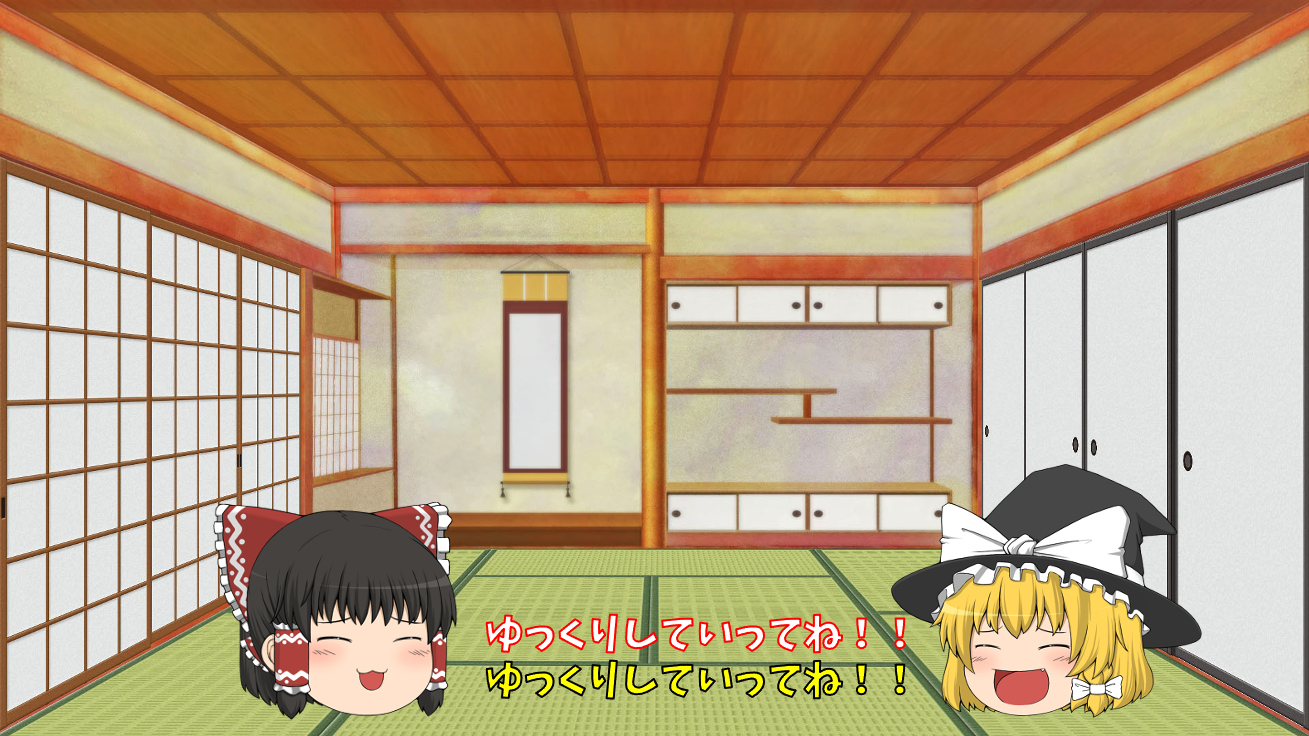
\includegraphics[width=6cm]{img-1.png}
  \caption{ゆっくりしていってね!!!}
\end{figure}
  おそらく一度は見たことがあると思うのですが、こちらは「ゆっくり」と呼ばれる謎の人頭饅頭です。現在、YouTube他多くのインターネット上のプラットフォームのあらゆる界隈に進出しており、「ゆっくり実況」「ゆっくり解説」「ゆっくり茶番劇」などの多彩な動画ジャンルを産んでいます。Googleで、「ゆっくり」のワードで動画検索をかけると、その数は約 35,200,000 件にも及びます。\\
実は、ゆっくりの誕生にもPC-98が深く関わっているのです。

ゆっくりには元ネタがあります。「れいむ」「まりさ」「さなえ」「ようむ」などの名前が何なのか気になって調べた人も中にはいるのではないでしょうか。ゆっくりはゲーム「東方Project」に登場するキャラクターが元になったものなのです。\\
それをインターネット掲示板「2ちゃんねる」(現5ちゃんねる)上の誰かが、人頭饅頭型の霊夢・魔理沙\footnote{どちらも東方Projectのキャラクターの一人です。}が「ゆっくりしていってね!!」と喋っているAA(アスキーアート)を作ったのが始まりです。\\
そしてなんと、元ネタとなったゲーム「東方Project」は、PC-98のゲームなのです。\footnote{東方Project第1弾~第5弾までが、PC-98上で動作するように作られました。}\\
PC-98中期~後期には、それまで企業や一部の物好きな金持ちのものだったコンピュータが、一般家庭にも普及し始めました。その中で、PC-98は東方Projectをはじめとする多くのゲームや音楽などを通して、日本のサブカルチャーの発展に大きな影響を与えたのです。PCとそれに関わる大衆文化について考えるには、PC-98の歴史を知ることが不可欠、と言えるでしょう。
\part{98の何がいいの?}
\setcounter{section}{0}
さて、ここまでの文章を読んですでに読者の皆様は「早くPC-98について教えてくれよ!!!!」と期待絶頂であるかと推察いたしますが、いかがでしょうか(笑)\\

...え?

\begin{screen}
「98がすごいPCだということはまあわからんでもない。でも、そんな30年前の骨董品をいじって何が楽しいんだ?」
\end{screen}

...わかりました!!そこまで仰るのなら存分に語って差し上げましょう!!\footnote{このように、ヲタクと呼ばれる人種に不用意にこのような質問をすると長時間拘束される割合が極めて高いという事実が報告されておりますので、ぜひともご注意ください。}

というわけで、以下に自分がPC-98をいじる理由を列挙してみました。\\
\section[short]{純国産PC}
現代のPCは、主にどこの国で作られているかご存知ですか?\\
現在は、日本のメーカーのPCであってもやっているのは設計ぐらいで、内部パーツ、組み立て含めそのほとんどは中国や台湾などの国々で製造されています。\\
また、PCの基本設計も、前述したようにアメリカIBM社のPC/AT互換機を基にしています。\\
PC-98を始めとする今から30~20年前のPCは、日本のメーカーが独自に設計し、日本の工場で製造されていました。\\
PC-98はOSなど一部のソフトウェアこそMicrosoft社のもの\footnote{BASICやMS-DOS、MS-Windows(後述します)のことを指します。NECも漢字ROMやBIOSは完全自社開発ですが、SHARPのX68000シリーズのHuman68kなどOSも自社製のコンピュータもあります。}をもとにしていましたが、それでさえ自社のコンピュータで動作するように独自に改良を加えていました。\\
「日本製」って、憧れますよね。また現在のPCとは一味もふた味も扱い方が新鮮で面白いものです。\\
\section[short]{苦労への憧れ}
皆さんは、「インターネット老人会」というワードを知っていますか?\\
これは、インターネットの黎明期にインターネットを使い始めた人たちのことを指します。\\
彼らは、誰よりも先にインターネットというものを知り、それを使ってみて、時には問題を解決しながら、インターネットやPCを使いこなしていきました。そして、彼らがそれらの技術について知見を深め、利用者の輪を広げ、新しいものを発明してくることでインターネットは今や世界中の人々にとってなくてはならないものになっています。\\
彼らは、新しい技術に触れ、そこに無限の可能性を感じながらそれらを自分たちでいじることを楽しんでいたのです。
現在で例えるとすれば、ChatGPTや生成AIに色々な命令をしてみて、「今日はこんな事ができるようになった!!」「AIってすげえ!!」と言っている人たち、になるんでしょうか。\\
私はその先駆者たちに強く憧れを感じています。\\
新しい技術というものは、いつでも厳しい努力を必要とするものです。しかし、それらの苦労を楽しむという姿勢は、とても尊敬できるものです。\\
PC-98を扱うのも、現代のPCの何倍も難しいものです。しかし、その苦労を実際に体験してみることで、彼らのことを追体験できるのではないか、と思っています。
便利なツールが一つもない中でコンピュータを動かすにはコンピュータについての深い理解が必要となります。古いPCを扱うことで、現代では当たり前のように機械がやってくれることを自分でやることになりますが、それをすることでコンピュータについての理解が更に深まると思っています。\\
\section[short]{こまけぇこたぁいいんだよ!!}
ここまで散々語らせていただきましたが、はい。もういいじゃないですか。だってPC-98かっこいいじゃないですか。(殴\\
今までの理由も後付けで、自分ももはや何故PC-98に興味を持ち、いじりだしたかはよくわかりません。\\
でも、「好きなこと」って、そういうものだと思います。もう私はPC-98の虜です。好きでなければ、こんな長い文章を書こうとは思いません(汗)
\part{ハードの紹介}
\setcounter{section}{0}
随分と長い前置きが終わったところで...お待たせいたしました!早速PC-98についての紹介に入っていきたいと思います。
まずはハードウェアから。
\section[short]{機種を見分けよう 〜型番〜}
ひとくちに 「PC-9800シリーズ」と言っても、多種多様な製品があります。
PC-98には、ほぼずべて「PC-98」で始まるモデル名がついており、以降に続く英数字で各機種を見分けます。中では特別な愛称がついているものもあります。
\begin{figure}[H]
  \centering
  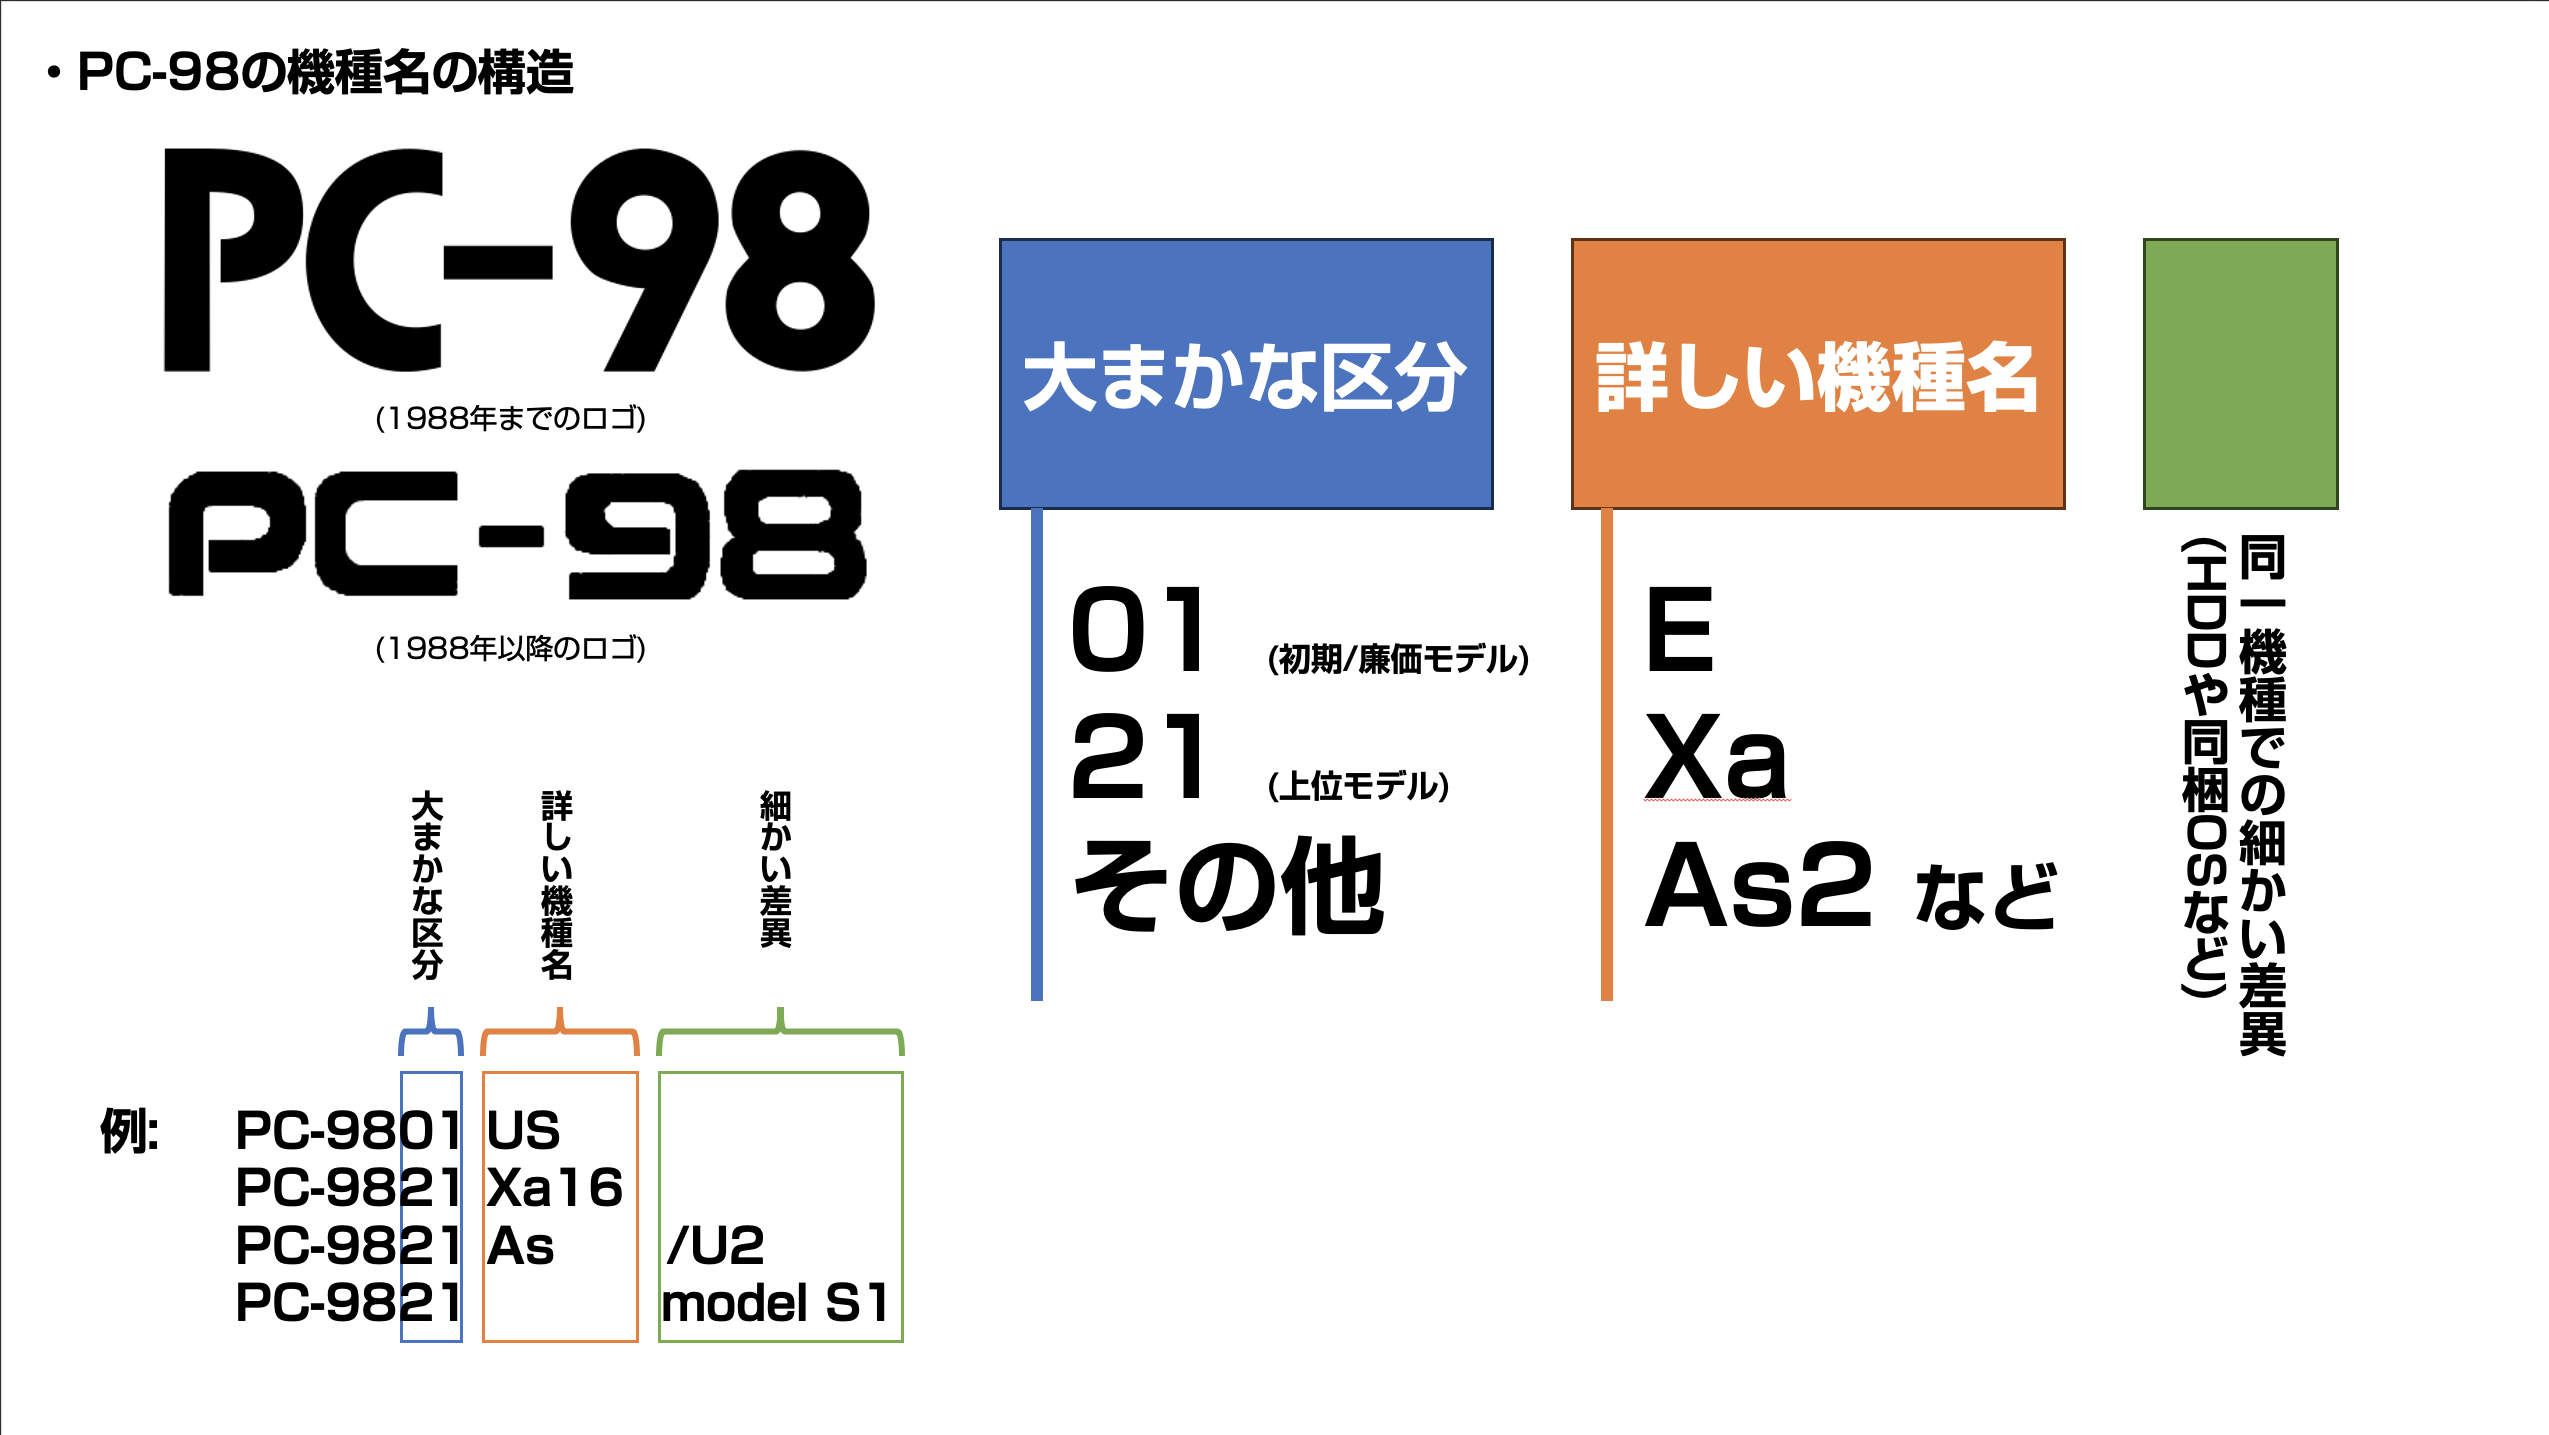
\includegraphics[width=5cm]{img-2.png}
  \caption{PC-98のモデル名(型番)の構造}
\end{figure}
まずPC-98の直後の「01」または「21」は大きなシリーズの差異を表します。\\
PC-9801は、PC-9800シリーズの中でも初期の製品群のことを指します。後述する「PC-9821」の登場までは、一部の特殊な製品を除いてPC-9800シリーズにはPC-9801型番しかありませんでした。\\
PC-9821は、1992年から登場したPC-9801の上位互換の製品群です。これによって、従来の「PC-9801」型番は、PC-9800シリーズの中で、廉価モデルや入門モデルの機種に付けられるようになりました。\\
その他では、PC-98LT(最初期のノートモデル)やPC-98XA(グラフィックス特化モデル)など、一部の特殊モデルには「PC-98」以下に01や21がつかない物があります\footnote{このような特殊モデルは、PC-9801を基本設計としながらも独自機能を多く搭載していたため、「PC-98」の名前を冠していながらも他機種との互換性が低く売上が伸び悩む傾向にありました。}。
次にその次に続く英数字は、その機種の詳細なモデルを指します。\\
モデルの中では、似た特徴を持つものに相性がつけられていることもあります。\\
モデル名の中でも有名なものを紹介します。\\
\begin{screen}
  PC-9821 As、Ap、Ae、An等Aがつくモデル...\\
  \ruby{MATE}{メイト} A シリーズ\\
  PC-9821 Cb、Cx、Ct、Cu等Cがつくモデル...\\
  98\ruby{MULTi}{マルチ} \ruby{CanBe}{キャンビー} シリーズ\\
  PC-9821 V13、V16、V20等Vがつくモデル...\\
  \ruby{VARUESTAR}{バリュースター} シリーズ
  \rightline{など}
  \end{screen}
  各機体の詳細は後述します。
\section[short]{PC-98を構成するパーツ}
さて、次にPC-98を構成するパーツについてご紹介します。とはいっても、その大部分は現代のPCと同じです。\\
最新のPCの情報も併記しておりますので、その違いを楽しんでいただければと思います。\\
全てについて説明するとみなさん速攻でこのページからオサラバしてしまいそうなので、ここでは各パーツの概要にのみ触れています。\\
興味が湧くパーツがあれば、ぜひとも調べてみてください。\\
好評であれば、次回はさらに深掘りしていきたいと思います。\\
\begin{enumerate}
  {\bf  \item CPU\\}
CPU(中央処理装置)は、コンピュータのまさにメインとなる、頭脳にあたる部分です。コンピュータの命令を解釈し、実行します。\\
PC-98には、主にIntel社製の「Intel 8086」とその後継及び互換CPUが搭載されています。\\
ちなみに、現在のIntel社のCPUはすべてIntel 8086の上位互換製品です。\\
CPUの速さは、そのCPUが一秒間に何回命令を実行できるかを表す「クロック周波数」で表されます。\\
現在のCPUは早いもので6GHz(1秒間に600億回)以上のクロック周波数を持っていますが、PC-98のCPUは5MHz(1秒間に500万回程度)から、早いものでも300MHzまででした。\\
こうして数字にしてみると、現代のCPUの方が圧倒的に早く、技術の進歩を感じさせられます。
今でこそ「遅い」と言えますが、当時からしてみれば100MHzを超えるCPUは高性能、300MHzなどは何でもできるスーパーマシンという認識でした。\\
\begin{itembox}[l]{主なCPU一覧}
  \begin{itemize}
    \item Intel 8086
    \item NEC V30
    \item Intel 80286
    \item Intel 80386
    \item Intel i486
    \item Intel Pentium
  \end{itemize}
\end{itembox}
  {\bf  \item メモリ(RAM)\\}
  メモリは、コンピュータが実行するプログラムやデータを一時的に保存する部分です。\\
  一時的に電気を貯めることのできる電子部品であるコンデンサを使って、情報を記憶します。\\
  その特性上、電源を切ると情報が消えてしまいますが、その代わり読み書きはハードディスクより高速に行うことができます。\\
  現在のPCでは、一般的にDIMMというメモリ(DDR4、DDR5という呼び方が一般的)が使われていますが、PC-98ではSIMMというメモリが一般に使われていました。\footnote{一部の末期のPC-9821ではDIMMが使えるものがありましたが、ほとんど普及していませんでした。}\\
  DIMMとSIMMの違いを簡単にいうと、SIMMが端子の両面とも同じ信号が流れていたのに対して、DIMMは片面ずつ異なる信号を流せるようになりました。つまり、DIMMはSIMMの2倍の情報をやり取りできるようになったということです。\\
  最近では8GBのメモリを搭載したPCがだんだん少なくなり、16GBが一般的になりつつありますが、PC-98では基本のメモリ640KB(0.00064GB)から始まり、拡張しても512MBなどがせいぜいといったところでした。しかも、増設しすぎると(プログラムがそこまでメモリがあることを想定していないために)プログラム側が誤動作する、ということもありました。\\
  {\bf  \item フロッピーディスク(FDD)\\}
  フロッピーディスクは、コンピュータが実行するプログラムやデータを一時的に保存するメディアです。\\
  磁気を帯びさせることができる円盤を回転させ、その上に磁気ヘッドを接触させることでデータを読み書きします。\\
  名前の「フロッピー」は、英語で「ぐにゃぐにゃした」という意味の「floppy」に由来します。\\
  手軽にデータを持ち運ぶことができるメディアとして、この時代広く用いられました。\\
  欠点は、データを記録する円盤の保護が甘く少しの傷や汚れ、衝撃でデータが消えてしまうことと、読み書きが遅いこと、そして容量が小さいことです。\\
  保存できるデータの量は360KB(2DD)、720KB(2HD)、1.2MB(2HD)、最大で1.44MB(2HD)でした。\\
  カッコ内の英数字は、フロッピーディスクへのデータの書き込み方法の種類を表します。\\
  例えば、2HDは両面高密度という意味で、ディスクの面裏それぞれに2倍のデータを書き込める、ということです。\\
  フロッピーディスクは、8インチ、5インチ(ミニフロッピー)、3.5インチ(マイクロフロッピー)の3種類がありました。\footnote{他にも多種多様なフロッピーのサイズが考案されましたが、定着したのは主にこの三種類のみです。}\\
  3.5インチフロッピーは、日本の大手メーカーであるソニーが開発したもので、現在でもフロッピーディスクのイメージとして定着しています。\\
  PC-98では、最初期の数モデルを除きすべての機種でフロッピーディスクドライブを搭載しています。\\
  最初期は外付けの8インチドライブ、初期から中期は内蔵の5インチドライブ、中期から末期は内蔵の3.5インチドライブが主流でした。\\
  現代ではフロッピーを実際に目にすることはほとんどなくなりましたが、長らくデータの持ち運び方法の主流であったために、PCソフトの保存アイコンに用いられたり、公官庁や金融機関ではいまだにフロッピーを使用する機器があるなどして問題になっていたりします。
  {\bf  \item ハードディスク(HDD)\\}
  ハードディスクは、コンピュータが実行するプログラムやデータを永続的に保存する部分です。\\
  電磁石の要領で、磁気を帯びさせることができる円盤を回転させ、その上に磁気ヘッドを接触させることでデータを読み書きします。\\
  その特性上、電源を切っても情報が消えることはありませんが、その代わり読み書きはメモリより遅く、また読み書きを繰り返すと円盤が傷ついてしまうことがあります。\\
  さて、PC-98では、初期ではHDDはオプションで、主にフロッピーディスクにデータを保存することを想定していました。
  容量も現代のものと比較してとても小さく、現代では1TB(1000GB)のものも珍しくありませんが、PC-98では20MBなどから最大で1GB程度まででした。\\
  PCとの接続のされ方(接続規格)も、今とは違います。
  今ではSATA (Serial ATA)が一般的ですが、PC-98では主に以下の規格が使われます。\\
  {\bf・\ruby{SASI}{サシ}(Shugart Associates System Interface)\\}
  SASIはShugart社(現在のSeagate社)が開発した規格で、HDDを2台まで接続できます。\\
  1社が開発した規格に乗っかる形で各社がPCやHDDに採用していたため、製品によって互換性がないことがありました。\\
  初期のPC-98の内蔵用として使われていましたが、すぐ後にIDEやSCSIに取って代わられました。\\
  {\bf・\ruby{SCSI}{スカジー}(Small Computer System Interface)\\}
  SCSIは、複数の機器を接続するための規格です。昔版のUSBといえば伝わりやすいでしょうか。\\
  デイジーチェーンと言って、数珠繋ぎにする形で複数の装置(PC含め最大8台)を接続することができました。\\
  PC-98では、内蔵用ではなく、外付け用として使われていました。\\
  Macintoshなど他のコンピュータでは、内蔵用としても使われていました。\\
  現在では、仕様を拡張、変更したSAS(Serial Attached SCSI)規格が、サーバー用として一部に残るのみです。\\
  {\bf・\ruby{IDE}{アイディーイー}(Integrated Drive Electronics、ATAとも)\\}
  IDEは、HDDまたはCDドライブを最大4台接続するための規格です。\\
  PC-98では、長期に渡り主に内蔵用として使われていました。\\
  外付けのSCSI、内蔵のIDEという形で長らく業界の標準でした。
  今ではこの仕様を拡張したSATA(Serial ATA)が一般的に使われるようになりました。\\
  {\bf  \item グラフィックアクセラレータ(GA)\\}
  グラフィックアクセラレータは、コンピュータが画像を描画するための部分です。\\
  画像を描画するための計算を高速化することで、より高解像度で、より多くの色数で、より高速に画像を描画できます。\\
  現代のPCでは、グラフィックボード(グラボ)やビデオカード、GPUと呼ばれるパーツになります。
  PC-98では、標準の画面描画機構にプラスして、主にWindows環境でゲームや動画再生などでより高速な描画を行うために、グラフィックアクセラレータが搭載されていました。\\
  {\bf  \item サウンドボード\\}
  サウンドボードは、コンピュータが音を出すための部分です。\\
  ゲームでBGMを出したりするにはまさに必須の部品で、サウンドカードを搭載することで、より高音質で、より多くの音を同時に出すことができます。\\
  PC-98に標準搭載されているのはビープ音と呼ばれる、ピーピーという音しか出せないものでした。\\
  そのため、ゲームや音楽を楽しむにはサウンドボードが必須でした。\\
  ほとんどの機種では何らかの音源を搭載していましたが、中には音源を搭載していない機種もあります。\\
  以下に音源の種類と、代表的なサウンドカードを示します。\\
  {\bf ・FM音源 \\}
  FM音源は、周波数変調合成音源と呼ばれる、周波数を変えることで音を出す方式の音源です。\\
  簡単にいうと、音が作り出す波に加工を加えて音を作り、その組み合わせで演奏する方式です。\\
  ゲームセンターなどで聞くことができる、ピコピコしながらもリッチな、まさにゲーム、といった音を出すことができます。\\
  PC-98では、主にYAMAHA社のOPN、OPNAというFM音源が使われていました。\\
  それを搭載したPC-9801-86というボードがとても有名で、PC-98のFM音源の事実上標準となっていました。\\
  このボード及びそれに準拠した音源の環境のことを「86音源」と言います。\footnote{ここでは便宜上あたかも「PC-9801-86が初めに出て、それに準拠したものが出てきた」ような書き方をしていますが、元々、PC-9801-86は前述のA MATEシリーズに内蔵の音源を、音源を搭載していない旧世代の機種で使えるように拡張ボードとして切り出したものです。}\\
  ちなみに、86音源はFM音源だけでなく、後述のPCM音源も搭載しています。\\
  {\bf ・PCM音源 \\}
  PCM音源は、パルス符号変調音源と呼ばれる、音の波形をそのまま記録する方式の音源です。\\
  簡単にいうと、音の波形をそのまま記録して再生する方式です。\\
  CDやMDなどの音楽メディアに使われている方式です。\\
  現代のPCでも一般的に使われている方式です。\\
  PC-98では後期のWindows環境でよく使われていました。\\
  {\bf ・\ruby{MIDI}{ミディ}音源 \\}
  MIDI音源は、MIDIという規格を使って音を出す方式の音源です。\\
  元々MIDIとは、楽器同士、楽器とコンピュータを接続するための規格です。\\
  楽器の持つ音の情報をコンピュータに送り、コンピュータがそれを解釈して音を出すことができます。\\
  ドの鍵盤をで弾いた、ドの鍵盤を離した、レの鍵盤を弾いた、などの情報が記録されます。\\
  MIDIの音を鳴らすには、MIDIのポートを増設するカードと、MIDI情報を解釈して音を出すシンセサイザーが必要です。\\
  MIDIには楽器情報と音階の情報などしか入っておらず、実際の音情報は入っていないため、解釈するシンセサイザーによって音色が変わります。\\
  当時はDTM\footnote{デスクトップミュージックの略。コンピュータを使って音楽を作ること。}をする人や、一部の音楽好き、ゲーム好きの間で広がりました。\\
  PC-98ではRoland社のGS音源、YAMAHA社のXG音源が存在し、2派が互いにしのぎを削っていました。\\
  \end{enumerate}
\end{enumerate}
\end{multicols*}
\end{document}
